\def\mySecNum{10.5}
\mySection{\mySecNum~American options}
%-------------- start slide -------------------------------%{{{ 1
\begin{frame}[fragile,t]

	At each node we use the following formula to compute the price:
	\begin{align*}
		P(S,K,t) = \max\left(K-S,e^{-rh}\left[P(uS,K,t+h)p^* + P(dS,K,t+h)(1-p^*)\right]\right)
	\end{align*}

	\begin{align*}
		p^* = \frac{e^{(r-\delta)h}-d}{u-d}
	\end{align*}
	\vfill

	Or simply

	\bigskip

	\begin{align*}
		P(S,K,t) = \max\left(K-S,\Delta S+B\right)
	\end{align*}
\end{frame}
%-------------- end slide -------------------------------%}}}
%-------------- start slide -------------------------------%{{{ 1
\begin{frame}[fragile,t]
\begin{center}
	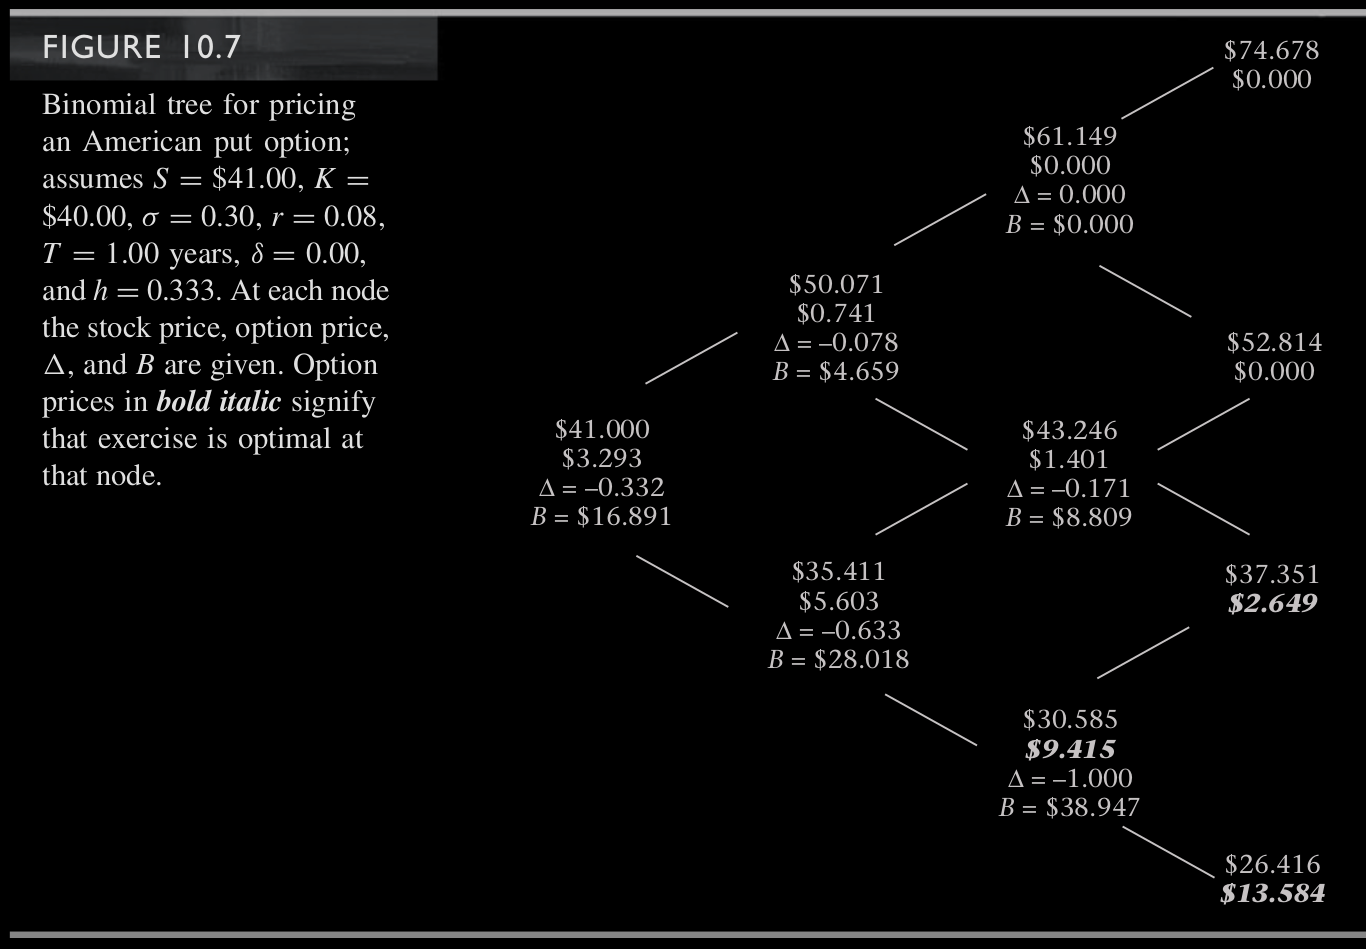
\includegraphics[scale=0.25]{figs/Figure-10-7.png}
\end{center}
\end{frame}
%-------------- end slide -------------------------------%}}}
